\documentclass[a4paper]{article}
\usepackage{graphicx}
\usepackage{xcolor}
\usepackage{dirtree}
\usepackage{tikz}
\usetikzlibrary{shapes,arrows}
\newcommand\myicn[1]{{\color{#1}\rule{2ex}{2ex}}}
\newcommand\mydir[3]{{\myicn{#1}\ {\textbf\large#2}:\ {\textnormal{\textit{\color{gray}#3}}}}}

\begin{document}
	\begin{titlepage}
		\includegraphics[width=0.5\textwidth]{logo.jpg}
		\par
		\centering
		\vspace{1cm}
		{\scshape\LARGE Z\'apado\v{c}esk\'a univerzita v Plzni\\Fakulta aplikovan\'ych v\v{e}d \par}
		\vspace{1cm}
		{\scshape\Huge Dokumentace k semestr\'aln\'i pr\'aci\\KIV/WEB\\Webov\'e str\'anky konferen\v{c}n\'iho
		syst\'emu \par}
		\vspace{1.5cm}
		{\Large\bfseries Martin \v{C}ervenka A14B0239P cervemar@students.zcu.cz \par}
		\vfill
		{\large 2. prosince 2016\par}
	\end{titlepage}
	\section{Pou\v{z}it\'e technologie}
		%uvedte hlavne, v ktere casti jste kterou technologii pouzili
		\begin{itemize}
			\item{HTML5}
			\item{CSS}
			\item{PHP}
			\item{MYSQL}
			\item{TWIG}
			\item{JS}
			\item{JQuery}
			\item{Bootstrap}
			\item{AJAX}
			\item{HTACCESS}
		\end{itemize}
	\clearpage

	\section{Adres\'a\v{r}ov\'a struktura}

		\begin{figure}[!ht]
			\dirtree{%
				.1 \mydir{black}{/}{Root directory}.
					.2 \mydir{red}{controller}{Soubory staraj\'ic\'i-se o funk\v{c}nost}.
						.3 \mydir{red}{js}{Obsajuje javascript(y) odes\'ilan\'e klientovi}.
						.3 \mydir{red}{twig}{Knihovna TWIGu}.
						.3 \mydir{white}{*.php}{Soubory zpracov\'avaj\'ic\'i p\v{r}\'ikazy od klienta}.
					.2 \mydir{blue}{doc}{Soubor(y) dokumetace}.
						.3 \mydir{white}{A14B0239P.pdf}{Tento soubor PDF}.
					.2 \mydir{green}{model}{Soubory pracuj\'ic\'i s daty}.
						.3 \mydir{white}{*.php}{Soubory pracuj\'ic\'i s daty}.
					.2 \mydir{yellow}{view}{}.
						.3 \mydir{yellow}{bootstrap}{Knihovna Bootstrapu}.
						.3 \mydir{yellow}{ckeditor}{Knihovna CKEditoru}.
						.3 \mydir{yellow}{templates}{\v{S}ablony TWIGU}.
							.4 \mydir{white}{*.tmpl}{Jednotliv\'e \v{s}ablony TWIGu}.
						.3 \mydir{white}{*.css}{Soubor(y) se styly}.
					.2 \mydir{orange}{texts}{Slo\v{z}ka pro uk\'ad\'an\'i dokument\r{u} PDF od klient\r{u}}.
					.2 \mydir{white}{.htaccess}{Nastaven\'i p\v{r}evodu ''p\v{e}kn\'ych'' URL adres}.
					.2 \mydir{white}{index.php}{Nastavuje TWIG a p\v{r}ed\'av\'a \v{r}\'izen\'i controlleru}.
			}
			\caption{Adres\'a\v{r}ov\'a struktura}
			\label{tree}
		\end{figure}
		\clearpage

	\section{Architektura aplikace}
		%co maji na starosti ktere tridy (popr. lze vyuzit i UML diagramy)
		\begin{figure}[!ht]	
			\centering
			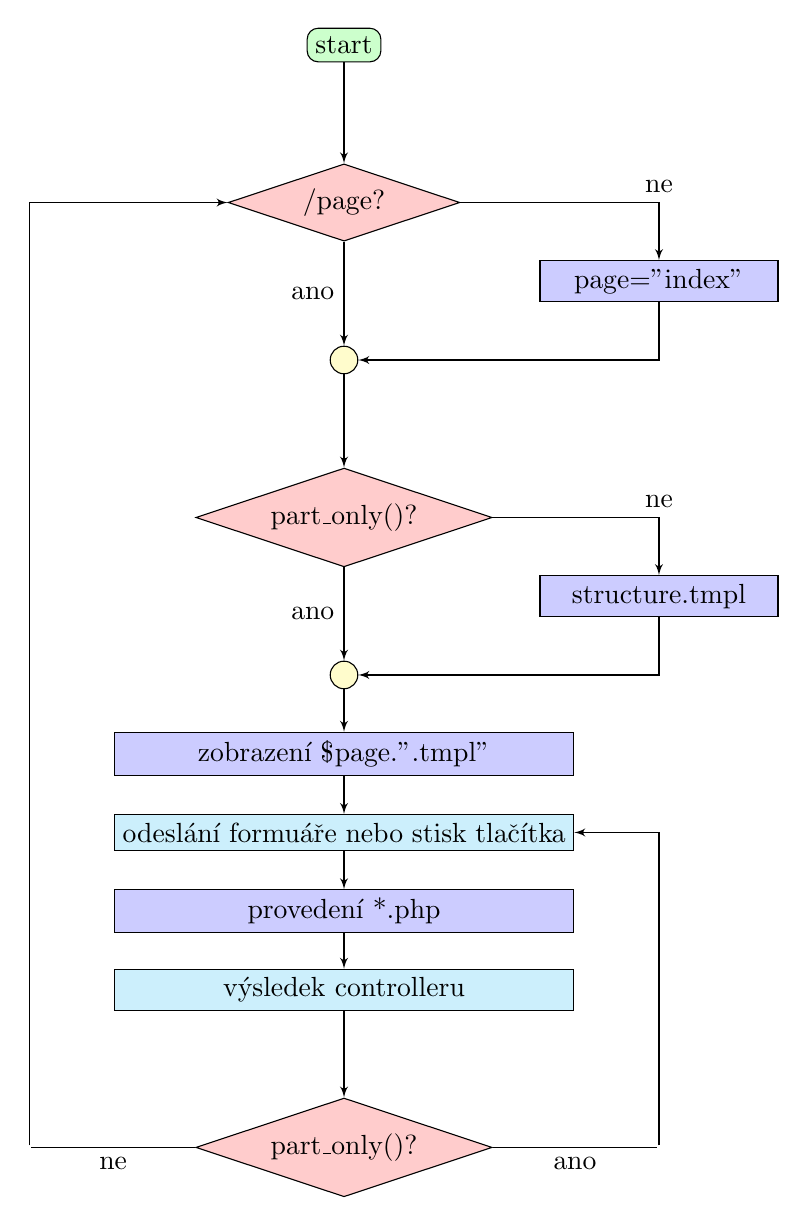
\begin{tikzpicture}
				\tikzstyle{common} = [draw, text badly centered, node distance=1cm and 2cm, inner sep=0.3em]
				\tikzstyle{decision} = [diamond, aspect=3, common, node distance=2cm, fill=red!20]
				\tikzstyle{cloud} = [rectangle, rounded corners, common, fill=green!20]
				\tikzstyle{block} = [rectangle, common, text width=16em, fill=blue!20]	
				\tikzstyle{block2} = [block, fill=cyan!20]
				\tikzstyle{merge} = [circle, common, fill=yellow!20, text width=1em ,inner sep=0]
				\tikzstyle{invisible} = [inner sep=0, draw=none, fill=none]
				\tikzstyle{line} = [draw, -latex']
				\tikzstyle{blockside} = [block, node distance=2cm, text width=8em]
				\node[cloud] (start) {start};
				\node[decision, below of=start] (page) {/page?};
				\node[invisible, below of=page] (i1) {};
				\node[merge, below of=i1] (merge1) {};
				\node[decision, below of=merge1] (part) {part\_only()?};
				\node[invisible, below of=part] (i2) {};
				\node[merge, below of=i2] (merge2) {};
				\node[block, below of=merge2] (pagetmpl) {zobrazen\'i \$page.".tmpl"};
				\node[block2, below of=pagetmpl] (input) {odesl\'an\'i formu\'a\v{r}e nebo stisk tla\v{c}\'itka};
				\node[block, below of=input] (control) {proveden\'i *.php};
				\node[block2, below of=control] (output) {v\'ysledek controlleru};
				\node[decision, below of=output] (po2) {part\_only()?};

				\node[invisible, node distance=4cm, right of=start] (top) {};
				\node[invisible, below of=top] (i3) {};
				\node[blockside, below of=i3] (setpage) {page="index"};
				\node[invisible, below of=setpage] (i4) {};
				\node[invisible, below of=i4] (i5) {};
				\node[blockside, below of=i5] (defpage) {structure.tmpl};

				\node[invisible, node distance=4cm, left of=po2] (x1) {};
				\node[invisible, node distance=4cm, right of=po2] (x2) {};
				\draw[line] (start) -- (page);
				\draw[line] (page) -| (setpage) node[midway,above]{ne};
				\draw[line] (page) -- (merge1) node[midway,left]{ano};
				\draw[line] (setpage) |- (merge1);
				\draw[line] (merge1) -- (part);
				\draw[line] (part) -| (defpage) node[midway,above]{ne};
				\draw[line] (part) -- (merge2) node[midway,left]{ano};
				\draw[line] (defpage) |- (merge2);
				\draw[line] (merge2) -- (pagetmpl);
				\draw[line] (pagetmpl) -- (input);
				\draw[line] (input) -- (control);
				\draw[line] (control) -- (output);
				\draw[line] (output) -- (po2);
				\draw[draw] (po2) -- (x1) node[midway,below]{ne};
				\draw[line] (x1) |- (page);
				\draw[draw] (po2) -- (x2) node[midway,below]{ano};
				\draw[line] (x2) |- (input);
			\end{tikzpicture}
			\caption{V\'yvojov\'y diagram}
			\label{img:diagram}
		\end{figure}
\end{document}
